\vspace{-10pt}
\section{Experimental Results}
\vspace{-5pt}

\begin{figure*}[t]
	\centering
	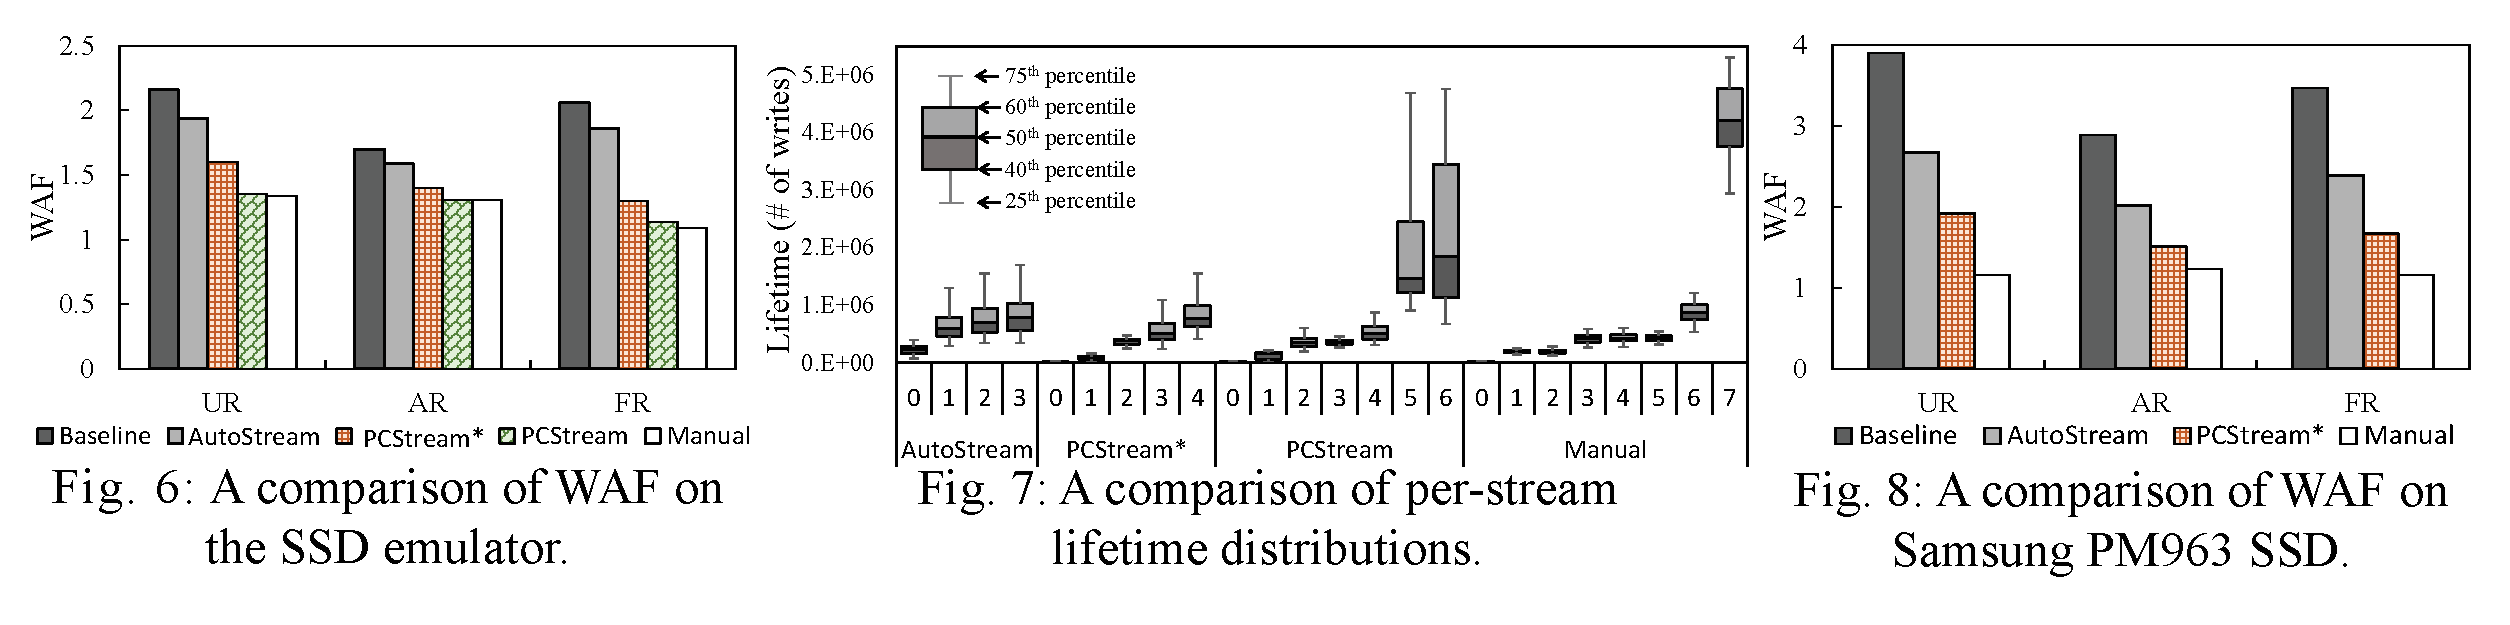
\includegraphics[width=1\textwidth]{figure/expfig}
%	\subfloat[\scriptsize{A comparison of WAF on the SSD emulator}.]{\label{fig:result_emul}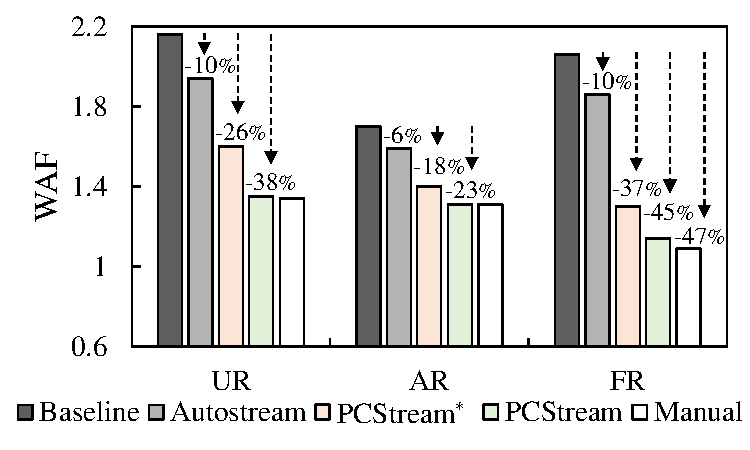
\includegraphics[width=0.33\textwidth]{figure/result_emul}}
%	\subfloat[\scriptsize{A comparison of WAF on PM963}.]{\label{fig:result_ssd}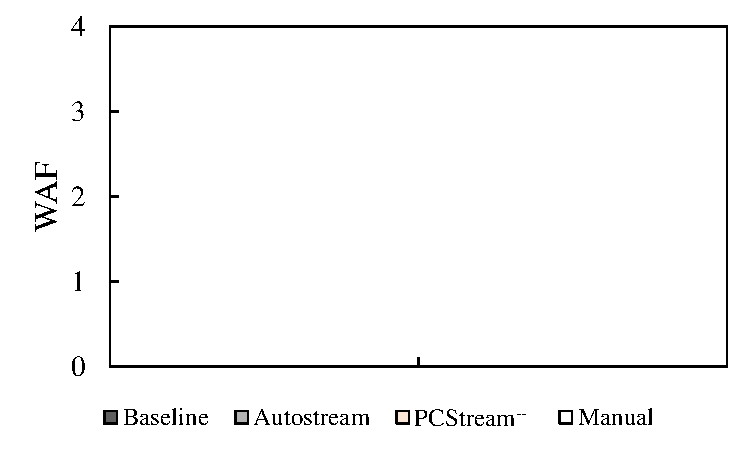
\includegraphics[width=0.33\textwidth]{figure/result_ssd}}
%	\subfloat[\scriptsize{A lifetime comparison of each stream}.]{\label{fig:streamlifetime}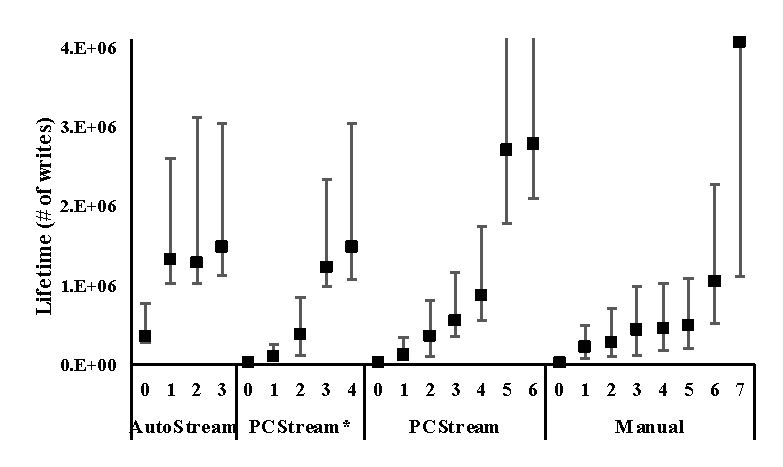
\includegraphics[width=0.33\textwidth]{figure/streamlifetime}}
%	\vspace{-10pt}
%	\caption{The WAF comparison on the emulator.}
	\label{fig:exp}
	\vspace{-35pt}
\end{figure*}

For our experiments, we have implemented \textsf{\small PCStream} in the Linux kernel
4.5.  For objective evaluation, we compared \textsf{\small PCStream} with three
existing schemes: \textsf{\small Baseline}, \textsf{\small Manual}~\cite{MultiStream}, and
\textsf{\small AutoStream}~\cite{AutoStream}.  \textsf{\small Baseline} stands for a legacy
SSD that does not support a multi-stream feature. \textsf{\small Manual} is a RocksDB
implementation which is manually optimized for multi-streamed SSDs.
\textsf{\small AutoStream} is an LBA-based data separation technique which is
implemented at the block driver layer. To understand the impact of the
two-phase assignment, in addition, we compared \textsf{\small PCStream} with
\textsf{\small PCStream$^{*}$} which excluded the two-phase assignment feature.

For benchmarks, we have used three scenarios of \texttt{db\_bench} of RocksDB:
Update-Random (\texttt{UR}), Append-Random (\texttt{AR}), and Fill-Random
(\texttt{FR}) scenarios.  For key-value pairs already stored in the SSD,
\texttt{UR} updates values for random keys, creating many
read-modify-writes in the SSD.  \texttt{AR} is similar to \texttt{UR}, except
that it performs the update of values for growing keys. \texttt{FR} writes
key-value pairs to the SSD in a random key order.

\vspace{-10pt}
\subsection{Experiments with an SSD emulator}
\vspace{-5pt}

\begin{comment}
\begin{figure}[t]
	\centering
	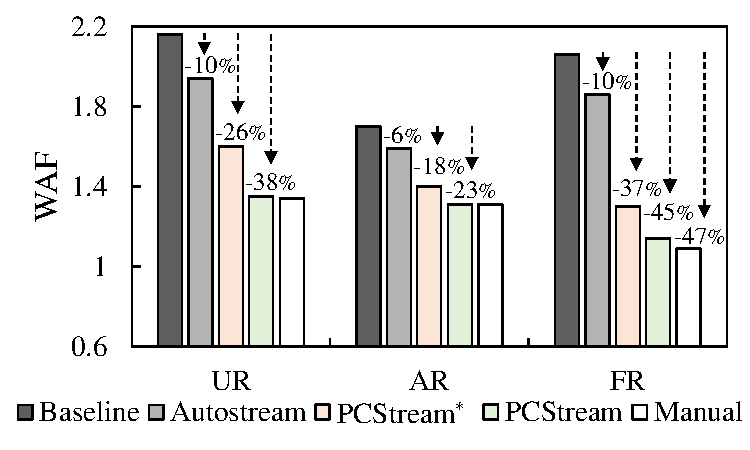
\includegraphics[width=0.8\linewidth]{figure/result_emul}
	\vspace{-10pt}
%	\caption{The WAF comparison on the emulator.}
	\caption{A comparison of WAF on the SSD emulator.}
	\label{fig:result_emul}
	\vspace{-15pt}
\end{figure}

 \begin{figure}[b]
	\centering
	\vspace{-15pt}
	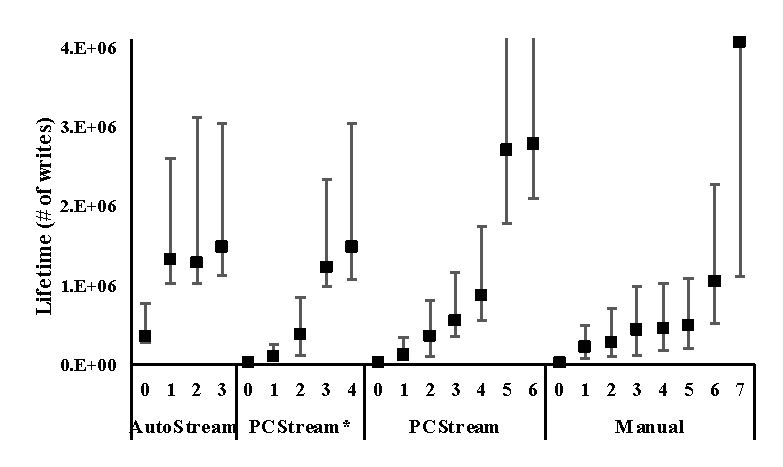
\includegraphics[width=1\linewidth]{figure/streamlifetime}
	\vspace{-20pt}
%	\caption{The WAF comparison on the emulator.}
	\caption{A lifetime comparison of each stream}
	\label{fig:streamlifetime}
\end{figure}

\begin{figure}[t]
	\centering
	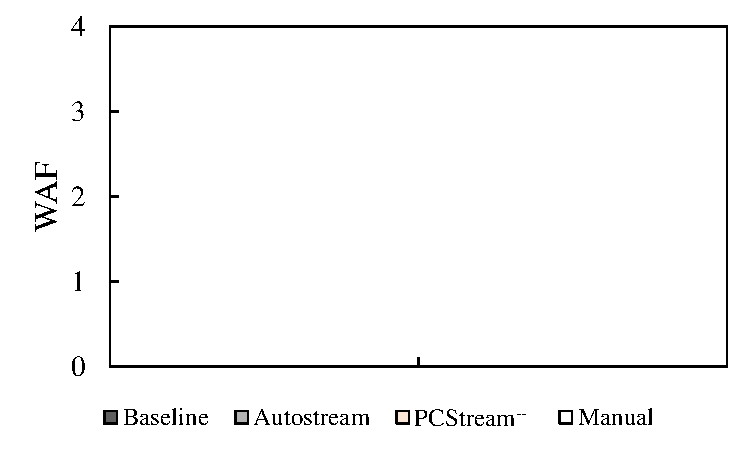
\includegraphics[width=0.8\linewidth]{figure/result_ssd}
	\vspace{-10pt}
	\caption{A comparison of WAF on PM963.}
	\label{fig:result_SSD}
	\vspace{-15pt}
\end{figure}
\end{comment}


We carried out a set of experiments using an SSD emulator which is based on the
open flash development platform~\cite{AMF}.  
%The SSD emulator emulates the behaviors of an SSD using host DRAM in the kernel level. Thus, it not only allows us to easily add new features, but enables to analyze detailed internal activities of an SSD. 
In the SSD emulator, the internal workings of an SSD is simulated using the host's DRAM memory in the kernel level. 
For our evaluations, we extended the SSD emulator to support a multi-streamed feature %.
(up to 8 streams). %shane part
Furthermore, we enhanced the garbage collection module of the SSD firmware to support the two-phase stream management technique. 
%We assume that the SSD emulator supports up to 8 streams (as with Samsung PM963 which was used in our experiments). %shane part
%We enhanced the original emulator so that it supported a multi-streamed feature as well as the two-phase stream assignment.  The number of streams supported by the emulator was 8.  
The SSD emulator provided 12 GB capacity with 4 channels and 4 ways, and there were 8192 flash blocks, each of which was composed of 384 4-KB pages.  


We compared WAF of the existing techniques with \textsf{\small PCStream} for the three
scenarios, and the result is shown in Fig. 6.  
\textsf{\small PCStream} was quite effective in reducing WAF, 
thus achieving an equivalent level of the WAF reduction as in \textsf{\small Manual}.  
For example, both \textsf{\small PCStream} and \textsf{\small Manual} reduced WAF by 38\% over Baseline for the \texttt{UR} case. 
Compared with \textsf{\small AutoStream}, \textsf{\small PCStream} was more effective, reducing WAF more by 35\% on average.  
Fig. 6 also indicates that the two-phase stream assignment technique is effective.  
\textsf{\small PCStream} outperformed \textsf{\small PCStream$^{*}$} by 12\% on average in the WAF reduction.
%As shown in Fig. 6, \textsf{\small PCStream$^*$} reduced WAF by up to 30\% over \textsf{\small AutoStream}.  
%The result shows that separating short-lived data (e.g., log and flush) from long-lived one (e.g., compaction) using PC was quite effective in reducing WAF.  Moreover, \textsf{\small PCStream} even showed similar WAF to \textsf{\small Manual}, reducing it by up to 38\% over \textsf{\small AutoStream}.  
This additional gain of \textsf{\small PCStream} over \textsf{\small PCStream$^{*}$} came from isolating long- and short-lived data in separate blocks through the two-phase assignment at the SSD even if they belonged to the same compaction PC.


In order to better understand how \textsf{\small PCStream} achieved a high reduction in WAF, 
we measured per-stream lifetime distributions under each technique for the \texttt{UR} scenario.
\textcolor{red}{
Fig. 7 shows a box plot of data lifetimes from 25\%-tile to 75\%-tile.}
%In order to analyze the improvement made by \textsf{\small PCStream}, 
%we measured the data lifetime of each stream for the {\tt UR} scenario.
%Fig. 7 shows average, 75p, and 25p of data liftime for each stream.
As shown in Fig. 7, 
streams in \textsf{\small PCStream} are divided into two groups, 
$G1$ and $G2$ where $G1$ includes streams with short lifetimes and small variances (e.g., streams 0, 1, 2, 3, and 4) 
and $G2$ includes streams with large lifetimes and large variances (e.g., streams 5 and 6).  
By preventing $G1$ and $G2$ from mixing in the same block, 
\textsf{\small PCStream} can reduce the GC overhead.  
On the other hand, in \textsf{\small AutoStream}, 
three streams (i.e., streams 1, 2, and 3) show similar lifetime distributions with large variances, 
thus not effectively taking full advantage of streams.
%data lifetimes of stream 0 to 5 in \textsf{\small Manual} are gathered in a narrow range so data lifetime in the same is quite similar.
%However, data lifetime of streams in \textsf{\small AutoStream} shows relatively large difference
%\textsf{\small AutoStream} does not notice when long-lived data is written to the hot stream.
%On the other hand, \textsf{\small PCStream$^*$} can identify short-lived data from 
%several dominant I/O activities as mentioned in section 2, for example, stream 0 and 1 in the Fig. 7.
%\textsf{\small PCStream} can further separate long-lived data of several streams (e.g., stream 3 and 4)
%by moving their data to substreams (e.g., stream 5 and 6, respectively). 
In Fig. 7, we can also observe the effect of substreams.  
Streams 3 and 4 of \textsf{\small PCStream$^{*}$}, 
which have large variances in lifetimes, are split into two substreams 5 and 6 in \textsf{\small PCStream}.
This split reduces variances of streams 3 and 4, thus improving WAF. 

\vspace{-10pt}
\subsection{Experiments with a real-world SSD}
%\vspace{-5pt}


In order to confirm the feasibility of \textsf{\small PCStream}, we also have
conducted experiments using Samsung's PM963 480GB SSD that supports 8 streams.
Since it was impossible to implement the two-phase stream assignment in the
commercial SSD firmware, we evaluated \textsf{\small PCStream$^*$} only.  To warm up the
SSD before running benchmarks, we filled up 90\% of the SSD capacity with valid
data.
As illustrated in Fig. 8, \textsf{\small PCStream$^*$} reduced WAF by
28\% over \textsf{\small AutoStream} on average.  
%There were large WAF gaps between \textsf{\small PCStream$^{*}$} and the manually optimized case.  If the substream was properly supported during GC, we believe that \textsf{\small PCStream} could show similar WAF values as \textsf{\small Manual}.  
Note that although \textsf{\small PCStream$^*$} still outperformed \textsf{\small AutoStream} in PM963, 
but a performance gap was smaller over that
in the emulated SSD environment.  It was difficult to pinpoint why
\textsf{\small AutoStream} worked better in PM963 over in the emulated SSD, but we
suspect that some internal features of PM963 (such as a large block size or some implementation details of streams) %might be related. 
might have affected the performance of \textsf{\small AutoStream}.

